\documentclass{report}
\usepackage[utf8]{inputenc}
\usepackage{amsmath}
\usepackage{biblatex}
\bibliography{refs.bib}
\usepackage{hyperref}
\usepackage{booktabs}
\usepackage{float}
\usepackage{enumitem}
\usepackage{amssymb}
\usepackage{graphicx}
\usepackage{pdflscape}
\usepackage{amsthm}
\usepackage{amsfonts}
\usepackage{bbm}
\usepackage{booktabs}
\usepackage{chngpage}
\usepackage[caption = false]{subfig}


\theoremstyle{definition}

% \newenvironement{news}{}{}

\title{CredibleCrowd: Empirical Mechanism Design for Crowdsourced Fact-checking}
\author{Mohammad Yaghini\\Data Science Lab (DLAB)\\EPFL}
\date{June 2018 \\[4cm]

\includegraphics[width = 2cm]{dlab_logo.pdf} \hspace{4cm} 
\includegraphics[width= 4cm]{EPFL-Logo-CMJN.eps}
}

\newcommand{\nitem}[1][]{\item \textbf{#1:}}
\newtheorem{definition}{Definition}
\newtheorem{example}[]{Example}

\begin{document}

\maketitle
\tableofcontents

% \chapter{Introduction}

% \chapter{Notation}
% \begin{itemize}
%     \item Argument $a$: A single proposition that can either be true (1) or false (0), which can be checked using absolutely credible\footnote{Absolute credibility is necessary at this level of granularity. We assume that such an argument can either be verifiable or not. We forgo the unverifiable arguments and verify the rest which resolves into True (1) or False (0).} sources of knowledge.
%     \item Argument value $V(a)$: $a\longmapsto \{0 , 1\}$. 1 for True, 0 for False.
%     \item News value $V(a_1, ..., a_n)$:  $\{0, 1\}^n \longmapsto [0, 1]$ a function of $n$ argument values $a_1$ through $a_n$.
%     \item Worker $w$: An intelligent agent (in our context mainly a human or possibly a fact-checking organization) that can evaluate the value of arguments and estimate the value of a piece of news.
% \end{itemize}

% \chapter{Problem Statement}
% A fact-checking task $t$ is a news item with value $V(a_1,...,a_t)$, where each $a_i~i=1...t$ is a argument which is either true or false. We employ $M$ workers to estimate the news value $V$. These workers return estimates $\Hat{V}_1,...,\Hat{V}_M$, design a payment rule which incentivizes the workers to fact-check each argument and give their true estimates of V, i.e, their 

% \begin{align}
%     &\hat{V}_i = \frac{\sum_{j=1}^t  \hat{a}_{j, i}}{t} &i=1...m,
% \end{align}

% where $\hat{a}_{j,i}$ is the estimated value of argument $a_j$ by worker $w_i$.

% \chapter{Mechanism Design}
% \section{Voting}
% If we map each worker reported decision to 0 or 1 (for example using a simple threshold on 0.5), we can hold a majority vote among two candidates that satisfies several desirable properties:
% \begin{enumerate}
% \item The protocol is not dictatorial, i.e. one agent decides the outcome. 
% \item There is not some candidate who cannot win under any preference profile. 
% \item There is no situation where an agent has an interest to not vote according to its true preference, i.e. to manipulate the outcome by a non-truthful vote.

% \end{enumerate}

% We quickly loose these properties if we consider more than 2 alternatives. (Gibbard–Satterthwaite theorem)


% \section{Peer Fact Checking}
% Each worker $w$ is presented with piece of news to fact check. She does not have a binary (True, False) choice to make, because she too, may not be completely sure of veracity or falsity of the news. Instead, she gives a value between 0 (false) and 1 (truth). Using a ``proper scoring rule''\cite{properScoring} we can in theory ensure truthful responses If the correct answer becomes eventually known.\cite{swissnoise} 

% This last condition requires that we have ground truth about the veracity of the news. This might seem like a strong condition, and particularly hard to satisfy in the context of debated news pieces. However, using "Peer Prediction" \cite{boi:book}

\chapter{Overview}
\section{Introduction}
With the advent of new propagation media, like social media and internet news websites, detecting and combating misinformation and fake (or false) news has gained renewed interest. This interest has recently been intensified due to the major role that fake news campaigns played in recent political overturns.

Detecting false news is no easy task. Aside from technical difficulties, even defining what is fake or what is not, is a highly polarizing issue. Interestingly, opinion polarization is both the cause and the effect of fake news. In such a polarized environment, we need systems, rule and regulations to bridge the gap.

When parties stop arguing and agree to disagree, they head to the polling stations to \emph{vote}, with the promise that whatever may be the outcome, it is the ``wisdom of the crowd, '' and as such, should be respected. The question is why can't we settle our disputes about fake news through such a voting mechanism?

One might argue that holding a vote for every controversial piece of  news is economically unfeasible. Plus, a vote to determine the veracity of a claim which can be proved or disproved objectively given enough proof is unnecessary if not outright wrong.

While all these concerns are valid, they are so in an ideal world. One in which we have the resources to investigate every claim. The reality is far from it. We are bombarded with false information on a daily basis, and no person or agency can take up the responsibility of fact checking all of the news we consume. Even if there was such an agency, it could not have assumed a non-political, not partisan agency. Its decisions would have been called an ``alternative'' fact, and its conclusions would have thus been disregarded.

Automated fact-checking is a promising tool that would alleviate many of the aforementioned issues. Such a system --- while potentially expensive to create, setup and maintain --- is scalable. It can collect opinion of the masses on a wide variety of issues, and leverage this wisdom of the crowd with transparent rules that enjoy bipartisan support.

An automated fact-checking system can be built to \emph{extract expertise} and \emph{incentivize truthfulness and effortful work}. CredibleCrowd is such a system. 

\section{System Objectives}
\begin{enumerate}
    \item Detecting the fake news pieces
    \item Motivating the crowd to detect/report fake news
    \item Finding arguments for and against a fact-checking decision and initiating a conversation with added value in the process
\end{enumerate}

\section{Overview}
In Figure (\ref{fig:overview}) you can see the overview of the CredibleCrowd. While this is not an exhaustive list of features, it outlines a few key points regarding the design of the system:
\begin{enumerate}
    \item The system is designed based on cutting-edge research in the domain of mechanism design, cognition theory and behavioral studies and computer science. 
    \item It is fine-tuned by \emph{iterative experiments} discovering the interplay of different schemes of voting and truthful information solicitation in realizing the objectives of the system.
    \item The experiments will be designed to test theories in three main categories:
        \begin{enumerate}
            \item How does a mechanism (or a particular implementation of it) lends itself to the problem of fake new detection?
            \item How is the interplay of Voting and Truthfulness-ensuring mechanisms? Are the two working effectively together?
            \item Upon success of the last phase of experiments, next we would be interested to see how the addition of annotation, argument mining/discovery and online discussions would change the dynamics of the system. Is it upgrading or degrading the system performance?
        \end{enumerate}
\end{enumerate}

\begin{landscape}
\begin{figure}
    \centering
    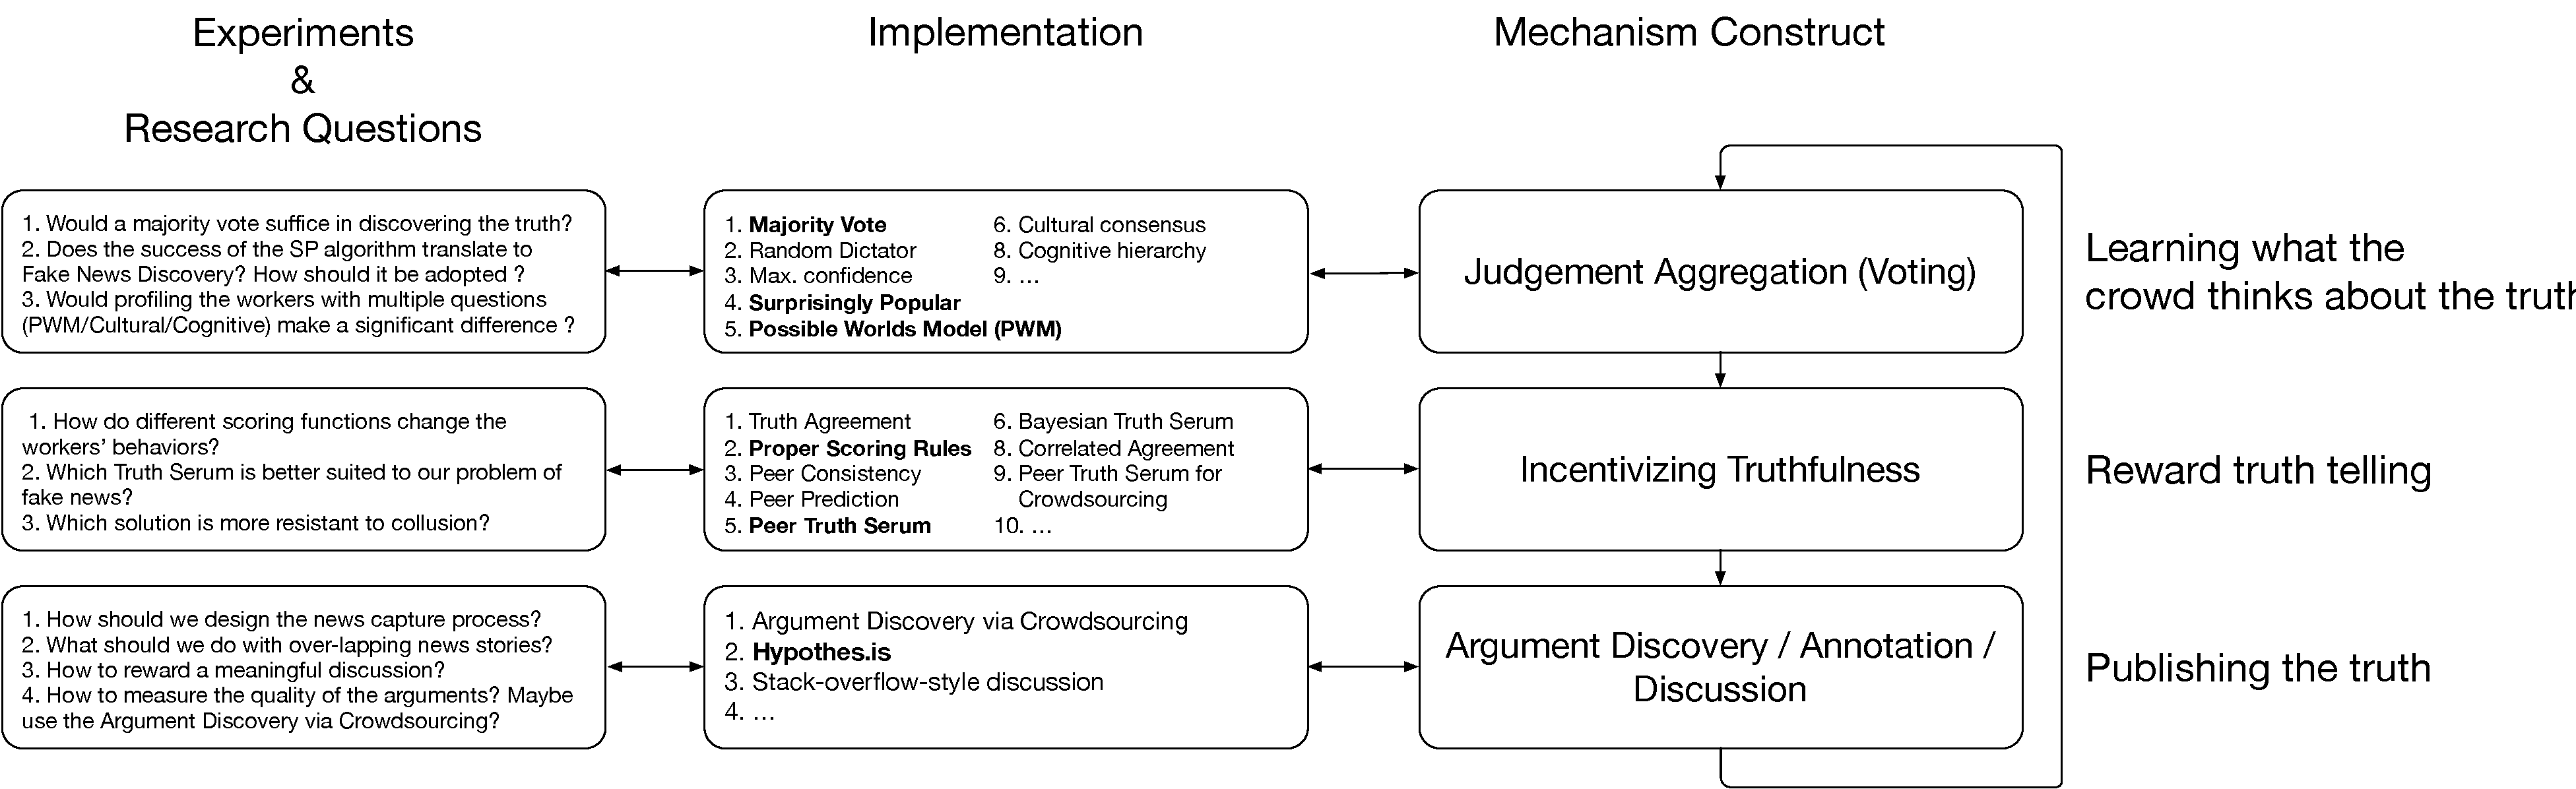
\includegraphics[width=1.8\textwidth]{fake_news_diagram.pdf}
    \caption{Overview of the CredibleCrowd mechanism construct, implementation methods and related experiments and research questions}
    \label{fig:overview}
\end{figure}
\end{landscape}



\chapter{Judgment Aggregation By Voting}
\begin{figure}[H]
    \centering
    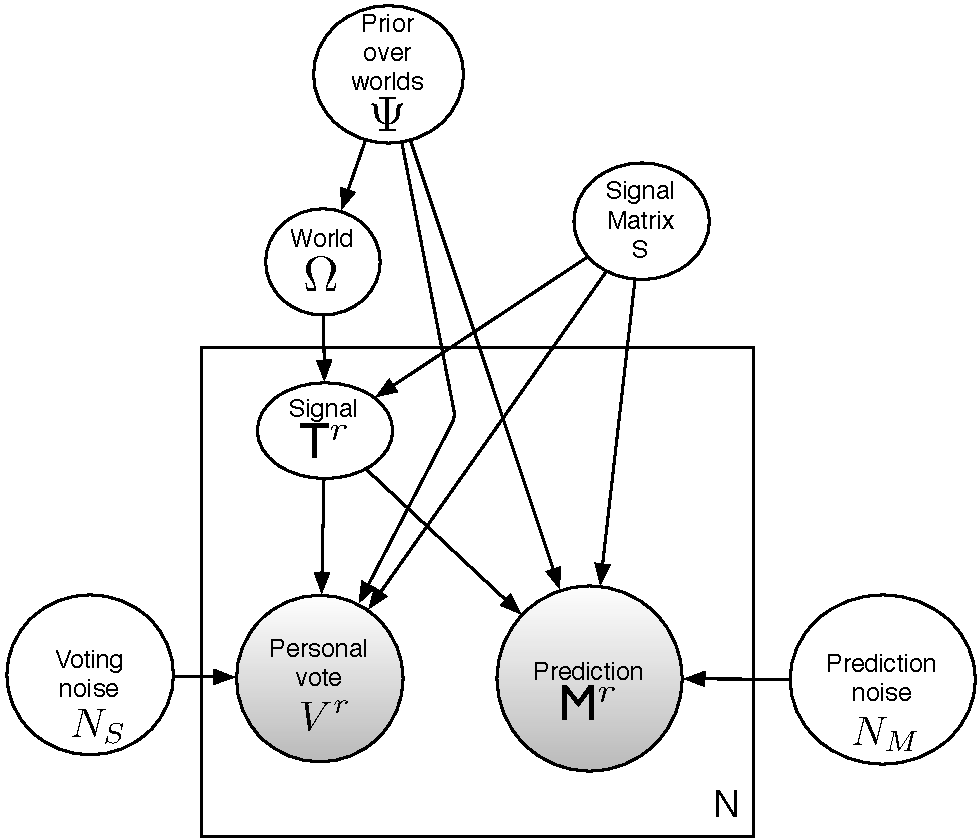
\includegraphics[width=\textwidth]{basic_generative_votes_updated.pdf}
    \caption{The single question possible worlds model (PWM) which is used to infer the underlying world state based on a group’s votes and predictions of the votes of others. In keeping with standard graphical model plate notation, nodes are random variables, shaded nodes are observed, an arrow from node X to node Y denotes that Y is conditionally dependent on X, a rectangle around variables indicates that the variables are repeated as many times as indicated in the lower right corner of the rectangle.}
    \label{fig:pwmsingle}
\end{figure}

\begin{figure}[H]
    \centering
    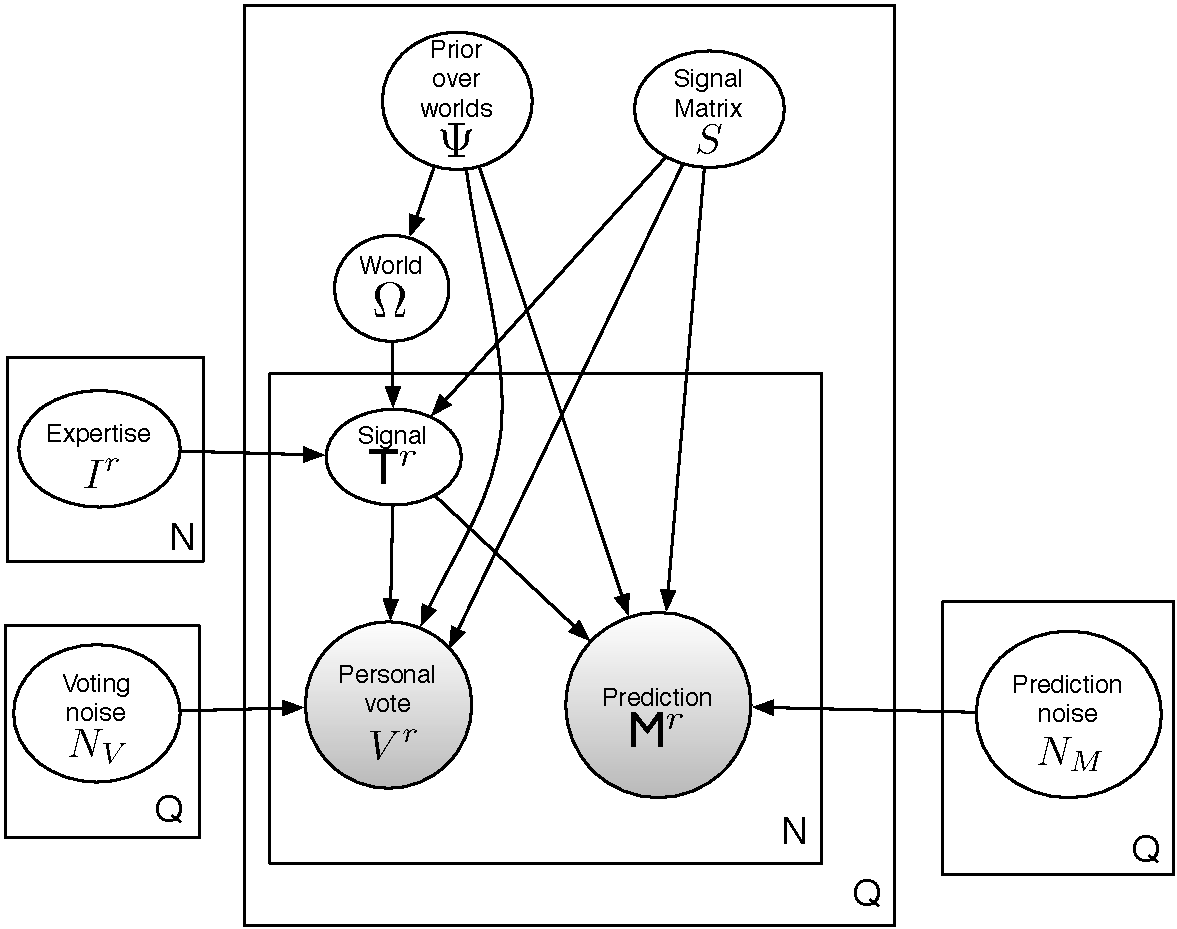
\includegraphics[width=\textwidth]{generative_individual_expertise_votes_updated.pdf}
    % \caption{The single question possible worlds model (PWM) which is used to infer the underlying world state based on a group’s votes and predictions of the votes of others. In keeping with standard graphical model plate notation, nodes are random variables, shaded nodes are observed, an arrow from node X to node Y denotes that Y is conditionally dependent on X, a rectangle around variables indicates that the variables are repeated as many times as indicated in the lower right corner of the rectangle.}
    % \label{fig:pwmsingle}
\end{figure}

\section{Surprisingly Popular}
\subsection{Example}
Imagine a piece of news. The world has a true state $\omega^* \in \Omega$ and  $\Omega = \{A, B\}$. There are two options $\{ \Tilde{A}, \Tilde{B}\}$. $\Tilde{A}$ and $\Tilde{B}$ are opposites: one says that the news is True, while the other says it is False (fake). It is assumed that in state $A$ answer $\Tilde{A}$ is the true answer, while in state $B$, answer $\Tilde{B}$ is correct.

The correct answer is not known, or equivalently, people do not know what is the true state $\omega^*$ of the world. However, it is assumed that if they knew, they would give a utility of 1 to the true answer and 0 to the other. 

A worker $w_i$ is given the piece of news and is asked to fact-check it. He uses the sources of information available to him or her, and receives a signal $s \in {a, b}$. 

Imagine that signal $a$ has probability 0.8
in state $A$ and probability 0.7 in state $B$ and thus be more likely
than signal $b$ in both world states. Under this signal distribution,
if the actual state was $B$ then the majority would receive signal
$a$, and, assuming a uniform common prior, would vote for state $A$
and so would be incorrect.

If the received signal is $a$ assuming that this signal has a uniform common prior, Then, its estimate of the
probability that the world is in state $A$ is $p(\Omega=A|s=a)=p(s=a|\Omega=A)p(\Omega=A)/p(s=a)=(.8)(.5)/((.8)(.5)+(.7)(.5))$
and since this quantity is higher than 0.5, workers receiving
signal $a$ vote that the world is most likely in state $A$. But
if the actual world is state $B$, workers have a .7 probability
of receiving signal $a$ and hence the majority of workers will
vote incorrectly.\cite{mccoy:stat}

However, using the Surprising Popular voting mechanism, after gathering the both the votes and predictions of the all the workers, we can see whether True or False has been more popular than expected in \emph{both} of the words. This, in turn, is our correct fact checking answer.

\section{Truthful people assumption}
In authors in \cite{mccoy:stat} and its preceding work \cite{prelec:nature} assume that people are truthful: ``people vote for the world state that they believe is most probable.'' In other words, they believe that eliciting truthful information via modifying the payment function is a separate task in designing voting mechanism. This suggestion is reflected in the separation of Voting and Truthfulness Incentivization submodules. In other words the Voting mechanism assumes truthfulness, and leaves the job of ensuring it to the latter submodule.



\chapter{Eliciting Truthful Information}
\section{Taxonomy and Categorization}

\begin{itemize}

\nitem[Center (Us)] Who collects the data from workers
\nitem[Data] 
\begin{itemize}
    \nitem[Objective] every agent observes the same realization of the phenomenon.
    \nitem[Subjective] each agent observes a possibly different realization of the same phenomenon.
\end{itemize}
\nitem[Center Goals]
\begin{itemize}
    \item Objective Data => Most Accurate Data
    \item Subjective Data => Obtain distribution of values observed by agents. 
\end{itemize}

\nitem[Verifiability]
\begin{itemize}
    \nitem[Verifiable] Center will eventually get access to the ground truth.
    \nitem[Unverifiable] There is no Ground Truth.
\end{itemize}
 
 \item (Worker) Strategies
 \begin{itemize}
     \nitem[Heuristic] reported value does not depend on an observation of the phenomenon.
     \nitem[Cooperative] the agent invests effort to observe the phenomenon and truthfully reports the observation.
 \end{itemize}
 
 \item Truthful Strategies
 \begin{itemize}
     \item Agents report their belief about the phenomenon truthfully.
     \item $\text{Cooperative} \subset \text{Truthful}$
 \end{itemize}
 
 \section{Crowd-sourced Fact Checking}
 \begin{itemize}
     \nitem[Objective Data] each task (news piece) has a state (True/False) that each worker observes and reports. \textit{Or} 
     \nitem[Subjective Data] each worker has a different belief about the veracity of a given task, and we want to correctly poll these opinions.
 \end{itemize}
  
\subsection{Why Peer Prediction makes sense in crowd-sourced fact checking?}

"The trick is that the common signal that allows the agents to coordinate their strategies is the phenomenon they can all observe."

The true signal (the phenomenon which a piece of news describes) should be the only coordinating signal among two workers. 


\section{What to strive for in a mechanism?}
\begin{itemize}
    \nitem [Truthfulness] induces agents to choose a cooperative and truthful strategy;
    \nitem[Individually Rational] where agents can expect a positive utility from participating;
    \nitem[Positive Self-selection] which means only agents that are capable of providing useful data can expect a positive utility from participating.
\end{itemize}

\section{Effort: The Need for Compensation}
\textbf{Monetary} such as actual money, reputation points, rewards, etc.


\textbf{Influence} or the leverage on the model that the center learns from data


\section{Belief: The agent's local information}
The belief of an information agent is characterized by a prior probability distribution 
\begin{equation}
    P_i(x) = {p_i(x_1), ..., p_i(x_n)}
\end{equation}
of what the state X of the phenomenon might be.

Following an observation, based on the received signal $s_i$ it will update its prior 
\begin{equation}
    P_i(X=x | S_i = s) = P_i(x|s)
\end{equation}
to a posterior distribution.

\subsection{Belief Update}
Belief update using Bayes Law
For \textbf{Objective} data, belief update should be  self-dominating: 	
\begin{definition} An agent's belief update is self-dominating if and only if the observed $o$ has the highest probability among all possible values $x$:

\begin{equation}
    q(o|o) > q(x|o), \forall x \neq o.
\end{equation}
\end{definition}
Ex.$\delta = 1/t$ would compute the moving average if $o$ is the $t$'th observation.

For Subjective data, it is enough for belief update to be self-predicting:
\begin{definition} An agent's belief update is self-predicting if and only if the observed $o$ has the highest relative increase in probability among  among all possible values:


\begin{equation}
    q(o|o)/p(o) > q(x|o)/p(x), \forall x \neq o.
\end{equation}
\end{definition}
\end{itemize}

\begin{example}
\begin{equation}
    \hat{q} = \begin{cases} 
(1-\delta)p(x) + \delta &\text{for } x=o \\
(1 - \delta)p(x)        &\text{for } x\neq o 
\end{cases} = (1 - \delta)p(x) + \delta.\mathbbm{1}_{x=o}
\end{equation}
\end{example}

\section{Summary}
See table (\ref{tab:summary}) for a summary of the relation between verifiability, objectivity the state of the Ground Truth and a couple of examples.

\begin{table}[]
\centering
\caption{Verifiability $\Longleftrightarrow$ Objectivity $\Longleftrightarrow$ Ground Truth}
\label{tab:summary}
\footnotesize
\begin{adjustwidth}{-4em}{}
\begin{tabular}{@{}llll@{}}
\toprule
Verifiability & Objectivity             & Ground Truth                                                                                                                                                                             & Example                                                             \\ \midrule
Verifiable    & Objective               & Always exists for the true value                                                                                                                                                         & \begin{tabular}[c]{@{}l@{}}Temperature \\ Measurements\end{tabular} \\
Unverifiable  & \begin{tabular}[c]{@{}l@{}}Objective\\
Subjective\\\end{tabular} & \begin{tabular}[c]{@{}l@{}}Doesn't exist for individual data (worker reports).\\ Exists for distribution of the reports. \\(Every worker samples from the same distribution.)\end{tabular} & Restaurant Reviews                                                 
\end{tabular}
\end{adjustwidth}

\end{table}


\section{Why Peer prediction wouldn't work as expected}

\begin{itemize}

    \item The main (very high-level) idea behind previous peer-prediction mechanisms can be understood as a “clever majority vote”—every agent is paid according to a specific similarity between her and her peer. Thus, they point out that in the peer-grading example, coordinating on just checking the grammar can guarantee good agreement with other agents, but with substantially reduced effort.\cite{kong:noverify}
    
    \item Gao et al point out that things are likely even worse than this. If the cheap signals correlate more than the expensive signals, then the peer-prediction techniques incentivize agents to not report the true answer, but instead focus on cheap signals! For example, in the essay grading above, it is likely that assessments of grammatical correctness will agree more than assessments of overall essay quality. Because of this, peer-prediction mechanisms will pay agents more overall for lower-quality information.\cite{kong:noverify}
    
    \item One approach to counter coordinated low-quality strategies is to use trusted agents that provide the correct answers for some randomly selected subset of tasks. In a hybrid mechanism, agents’ reports will be either compared to other agents, or to such trusted reports. If the probability of having a trusted agents as a peer is sufficiently high, other low-quality equilibria can be broken. However, It has recently been shown that if the coordinated low-quality strategy provides higher payoffs than the cooperative strategy (for example, because it involves no measurement noise), it may be better to use simple truth agreement rather than a combination with peer consistency mechanisms as a complement to the truthful reports.\cite{boi:book, gao:peer}
    
    \item An issue related to precision is the risk of agents coordinating on a signal other than the phenomenon itself, called low-quality signal in Gao et al.\cite{gao:peer}
\end{itemize}








\chapter{Experiments}
Since we are dealing with people and how they deal with spread of misinformation, we must base our mechanism on observations from real crowds. Therefore, we have designed and conducted experiments to gauge the performance of different models at each phase of the system.

The current work only deals with the first phase, ``Judgment Aggregation.'' Nevertheless, in the future work's section, we outline the design and requirements of  experiments for second and third phases.

\section{Experiment 1}
In this experiment, we want to answer these research questions:

\begin{enumerate}
    \item Would a majority vote suffice in discovering the truth?
    \item Does the success of the SP algorithm translate to Fake News Discovery? How should it be adopted ?
    \item Would profiling the workers with multiple questions (PWM/Cultural/Cognitive) make a significant difference ?  
\end{enumerate}

For this first experiment, we used the crowd-sourcing platform, Amazon Mechanical Turk (AMT). In AMT, a \textbf{requester} can post Human Intelligence Tasks (\textbf{HITs}) on a ledger, and MTurk \textbf{workers} with (optional) qualifications can accept the HIT and start working on this.

AMT is frequently used for tasks that are still onerous for machines to perform well, including labeling datasets etc. However, many researchers in varied fields from Human Cognition and Neuroscience to Psychology and Behavioral Studies, have been using AMT as a platform to perform controlled-experiments. In fact, these have become so frequent that separate platform have appeared to ease the process of conducting such experiments, such as \textit{psiTurk}.

\subsection{Experiment Setting}
For this experiment, to avoid an unbalanced dataset of answers, we designed a web-page HIT, where we asked our respondents to answer three questions about 11 news pieces that we have selected from a labeled dataset of fake news~\cite{allcott:stanford}:

\begin{enumerate}
    \item Is this news piece real or fake?
    \item How confident are you in your answer?
    \item What percentage of other American MechanicalTurk respondents do you think would answer "Real" to the first question?
\end{enumerate}

The respondents had to provide a percentage above 50\% for question 2, and a percentage between 0 and 100\% for question 3. Moreover, in order to ensure that respondents have read the article, and are not just filling out the form randomly, we ask a forth question about a \emph{honeypot} embedded in the text.

\paragraph{Honeypot} is a relatively easy riddle to be solved by respondents for validating their engaged (effortful) answers before continuing to the next question. It is embedded into the news text, as an out-of-context sentence about a semantically unrelated thing like a fruit. Honeypots are hard to recognize by a syntax- or style-minded parser, but are obvious to a semantic-minded one.

\paragraph{Remuneration and Bonuses} To replicate the experiment carried out by Prelec et. al in \cite{prelec:nature}, we decided to use an almost identical remuneration scheme to theirs. Therefore, the participants were paid a flat participation fee of \$2 for their participation in the 10-minute study regardless of their answers. Their expertise was awarded by separate bonuses on their accuracy of answers and estimation of others, with separate \$2 bonuses to the top 20\%.

\begin{figure}[H]
    \centering
    \vspace*{-2cm}
    \makebox[\linewidth]{
    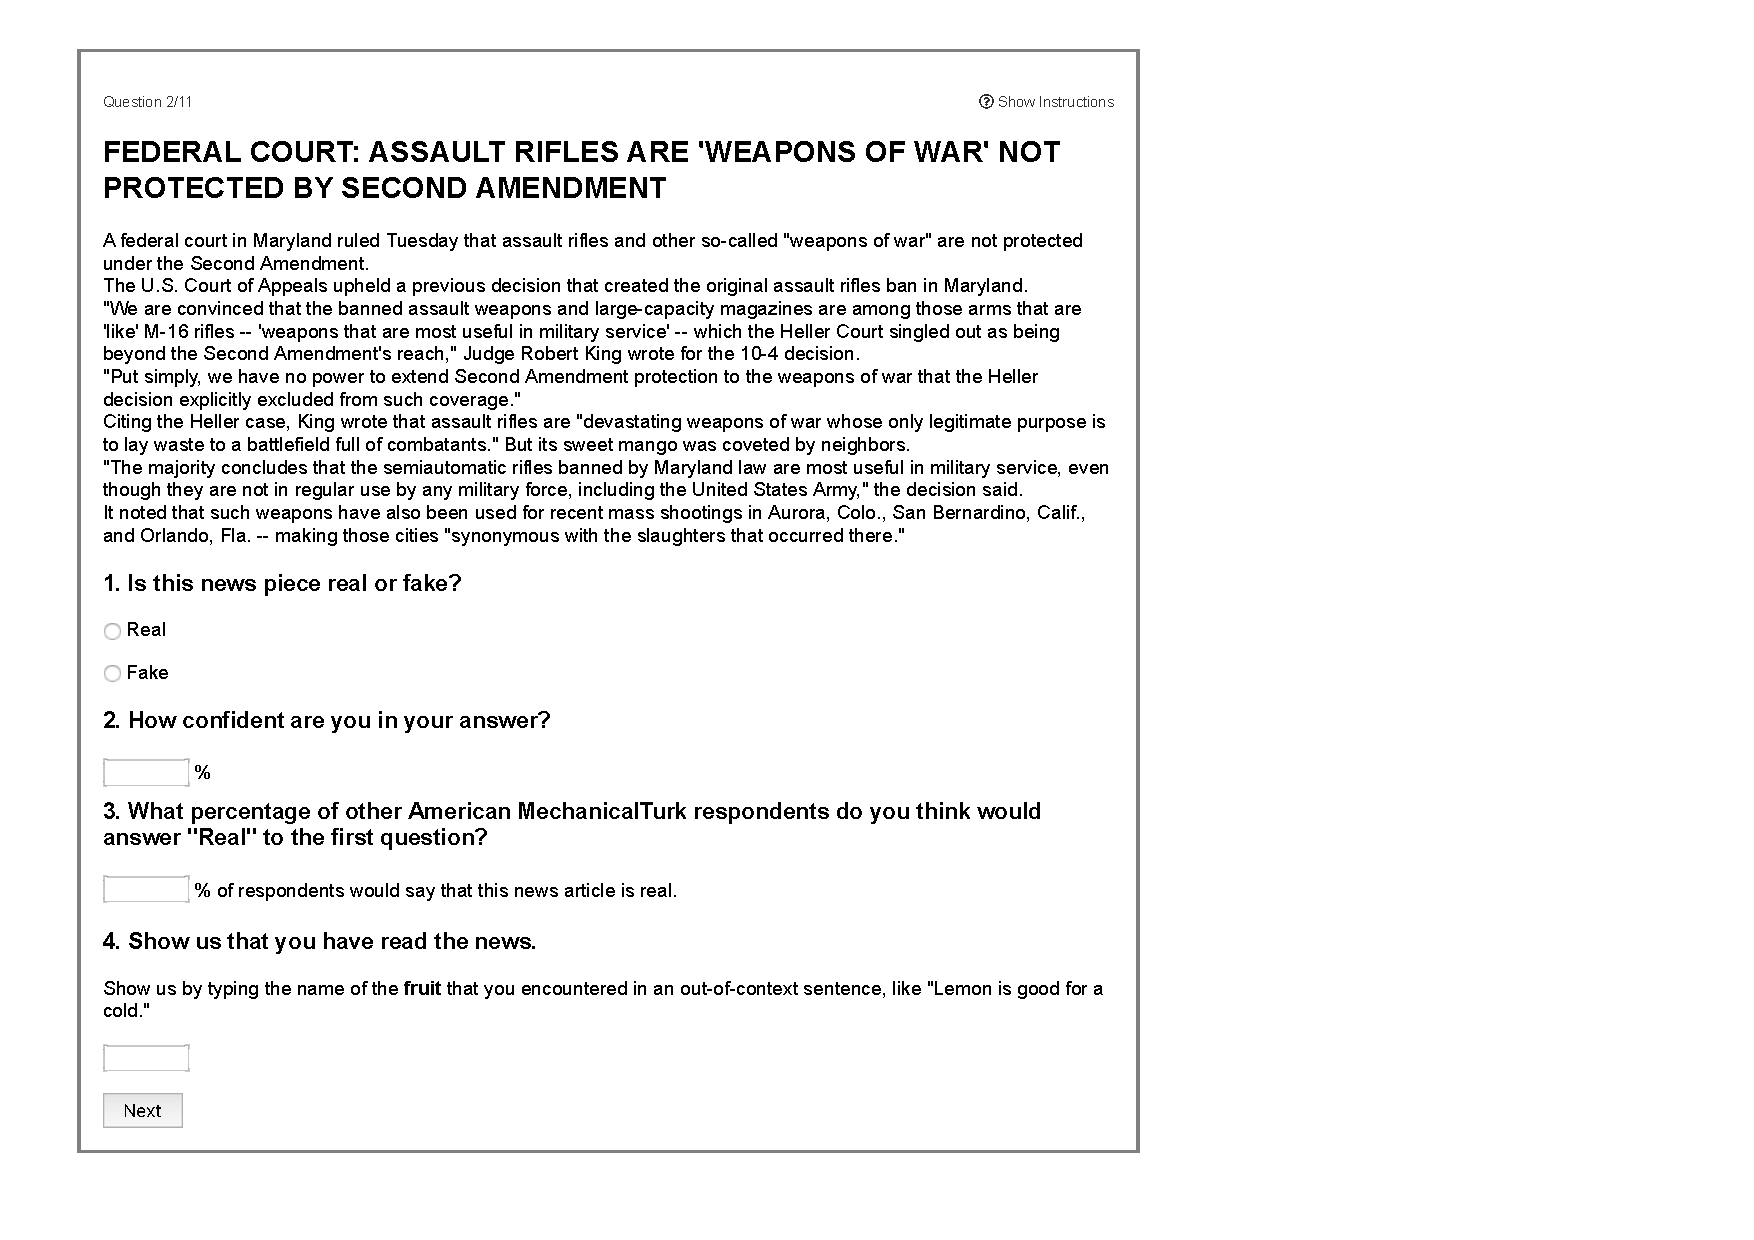
\includegraphics[width=1.5\textwidth]{experiement_sample_question.pdf}
    }
    \caption{Sample question from Experiment 1}
    \label{fig:sample_question}
\end{figure}


\newpage
\thispagestyle{empty}
\begin{figure}[H]
    \centering
    \vspace*{-4.2cm}
    \makebox[\linewidth]{
    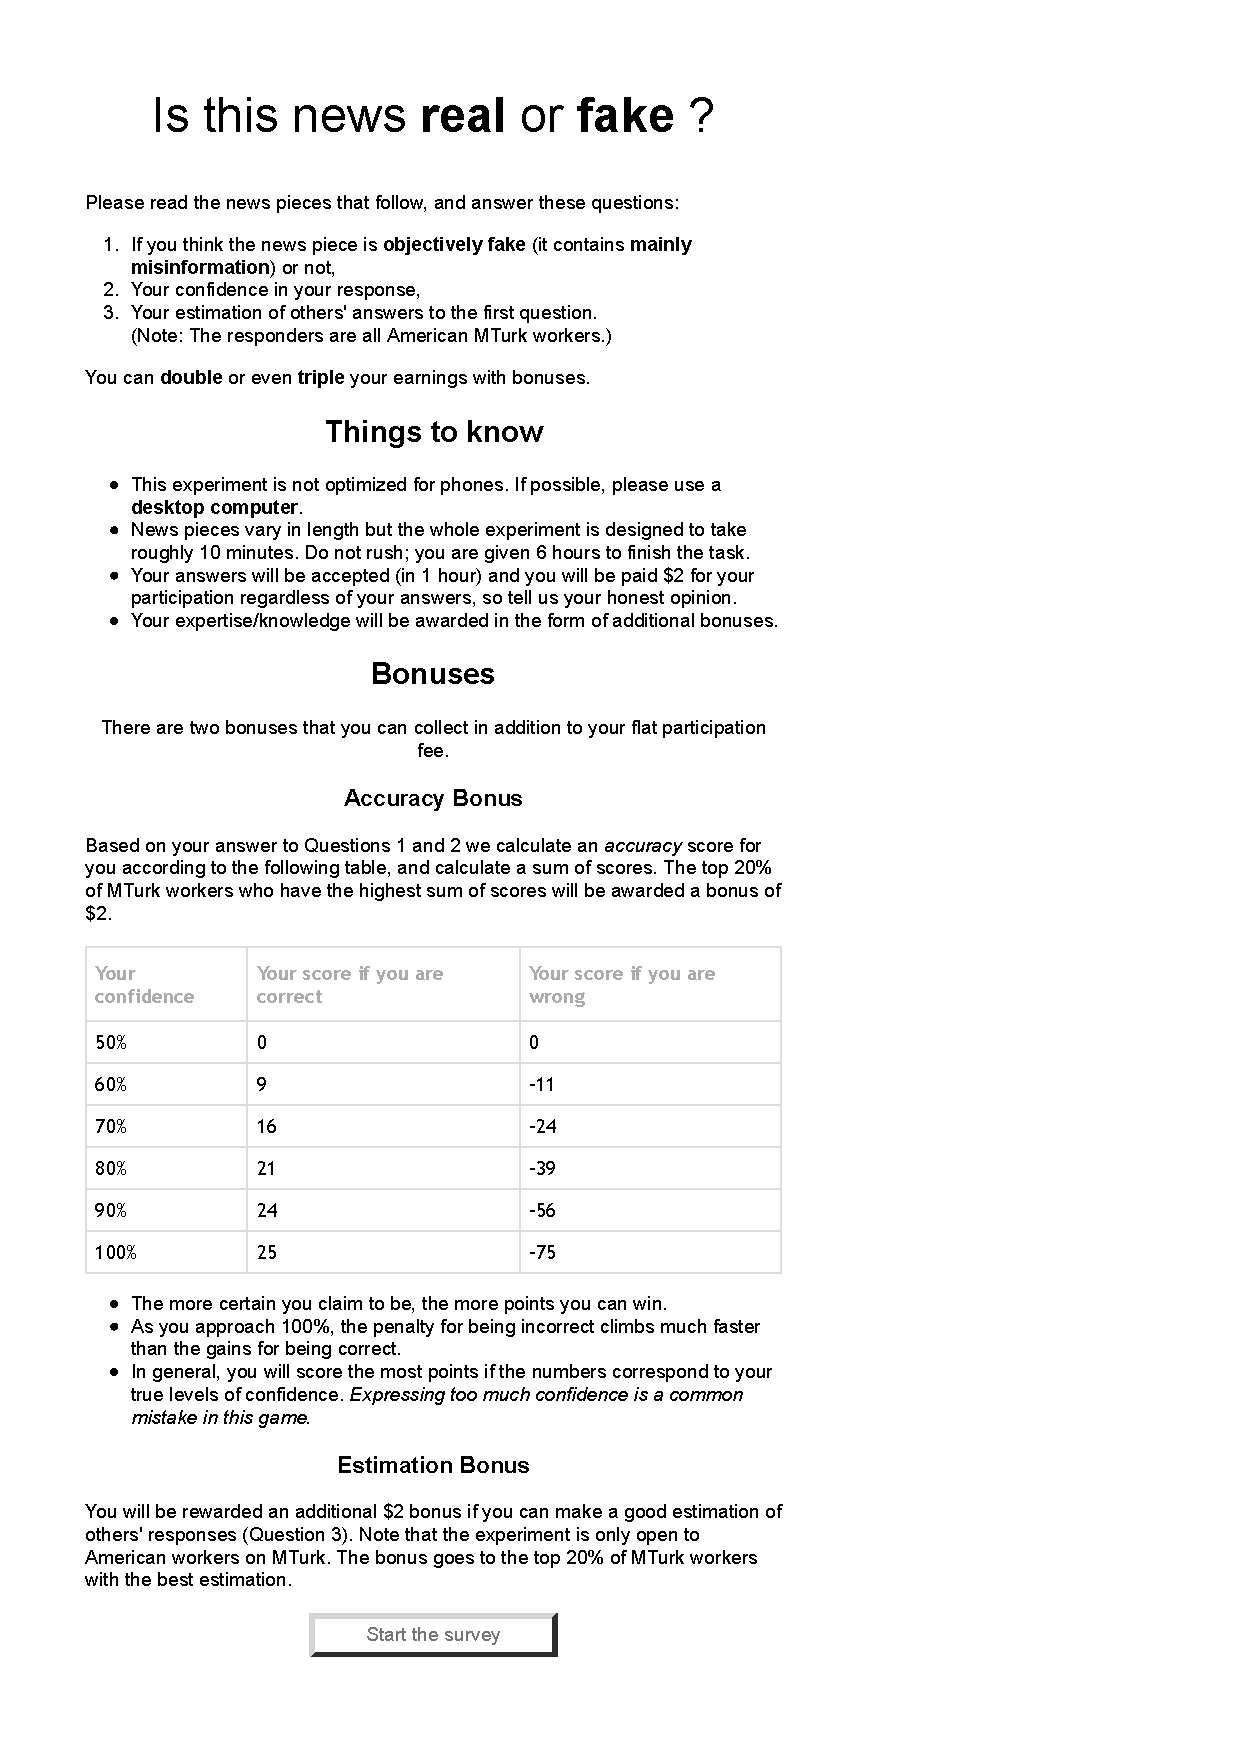
\includegraphics[trim={0 0cm 0 0cm}, clip, width=1.1\textwidth]{true_fake_first_page.pdf}
    }
    \caption{Instructions Page for Experiment 1}
    \label{fig:first_page}
\end{figure}



\subsection{Results}
50 participants took part in the experiment. 3 of the respondents submitted the experiment prematurely and as such their data was removed from the dataset.

\subsection{Accuracy}
The experiment contained 8 fake news articles and 3 real ones. Respondent's are not accurate on average (Figure \ref{fig:exp1_acc}). The majority of answers 
\begin{figure}
    \centering
    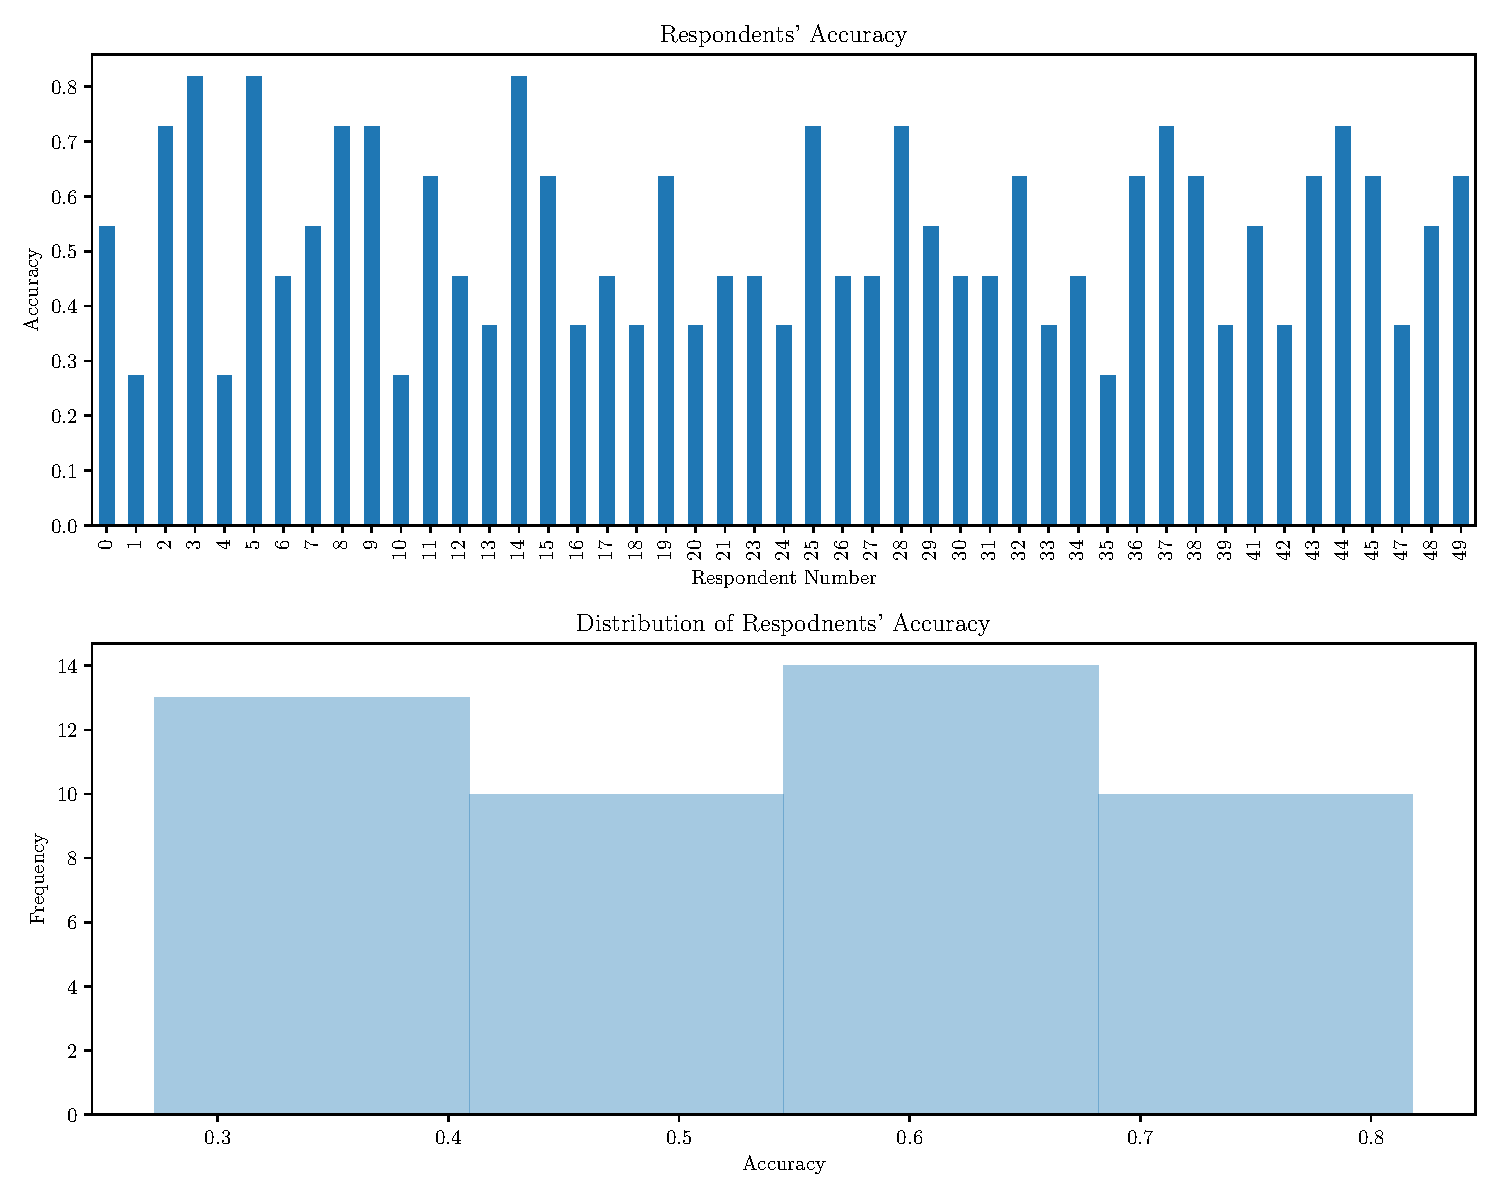
\includegraphics[width=\textwidth]{exp1_accuracy.pdf}
    \caption{AMT Respondents are not very accurate. The mean accuracy is just 53\%.}
    \label{fig:exp1_acc}
\end{figure}




\subsection{Confidence}
Figure \ref{fig:conf_hist} shows the histogram of confidences expressed by respondents in each trial. We observe a wide range of confidences in most trials. For most of the trials, the reported confidence seems very uninformative. Indeed, as we see in section \ref{sec:cwmv}, weighting the majority vote with the confidences expressed makes no difference in the performance of the voting scheme.

\begin{figure}[H]
    \centering
    \makebox[\linewidth]{
    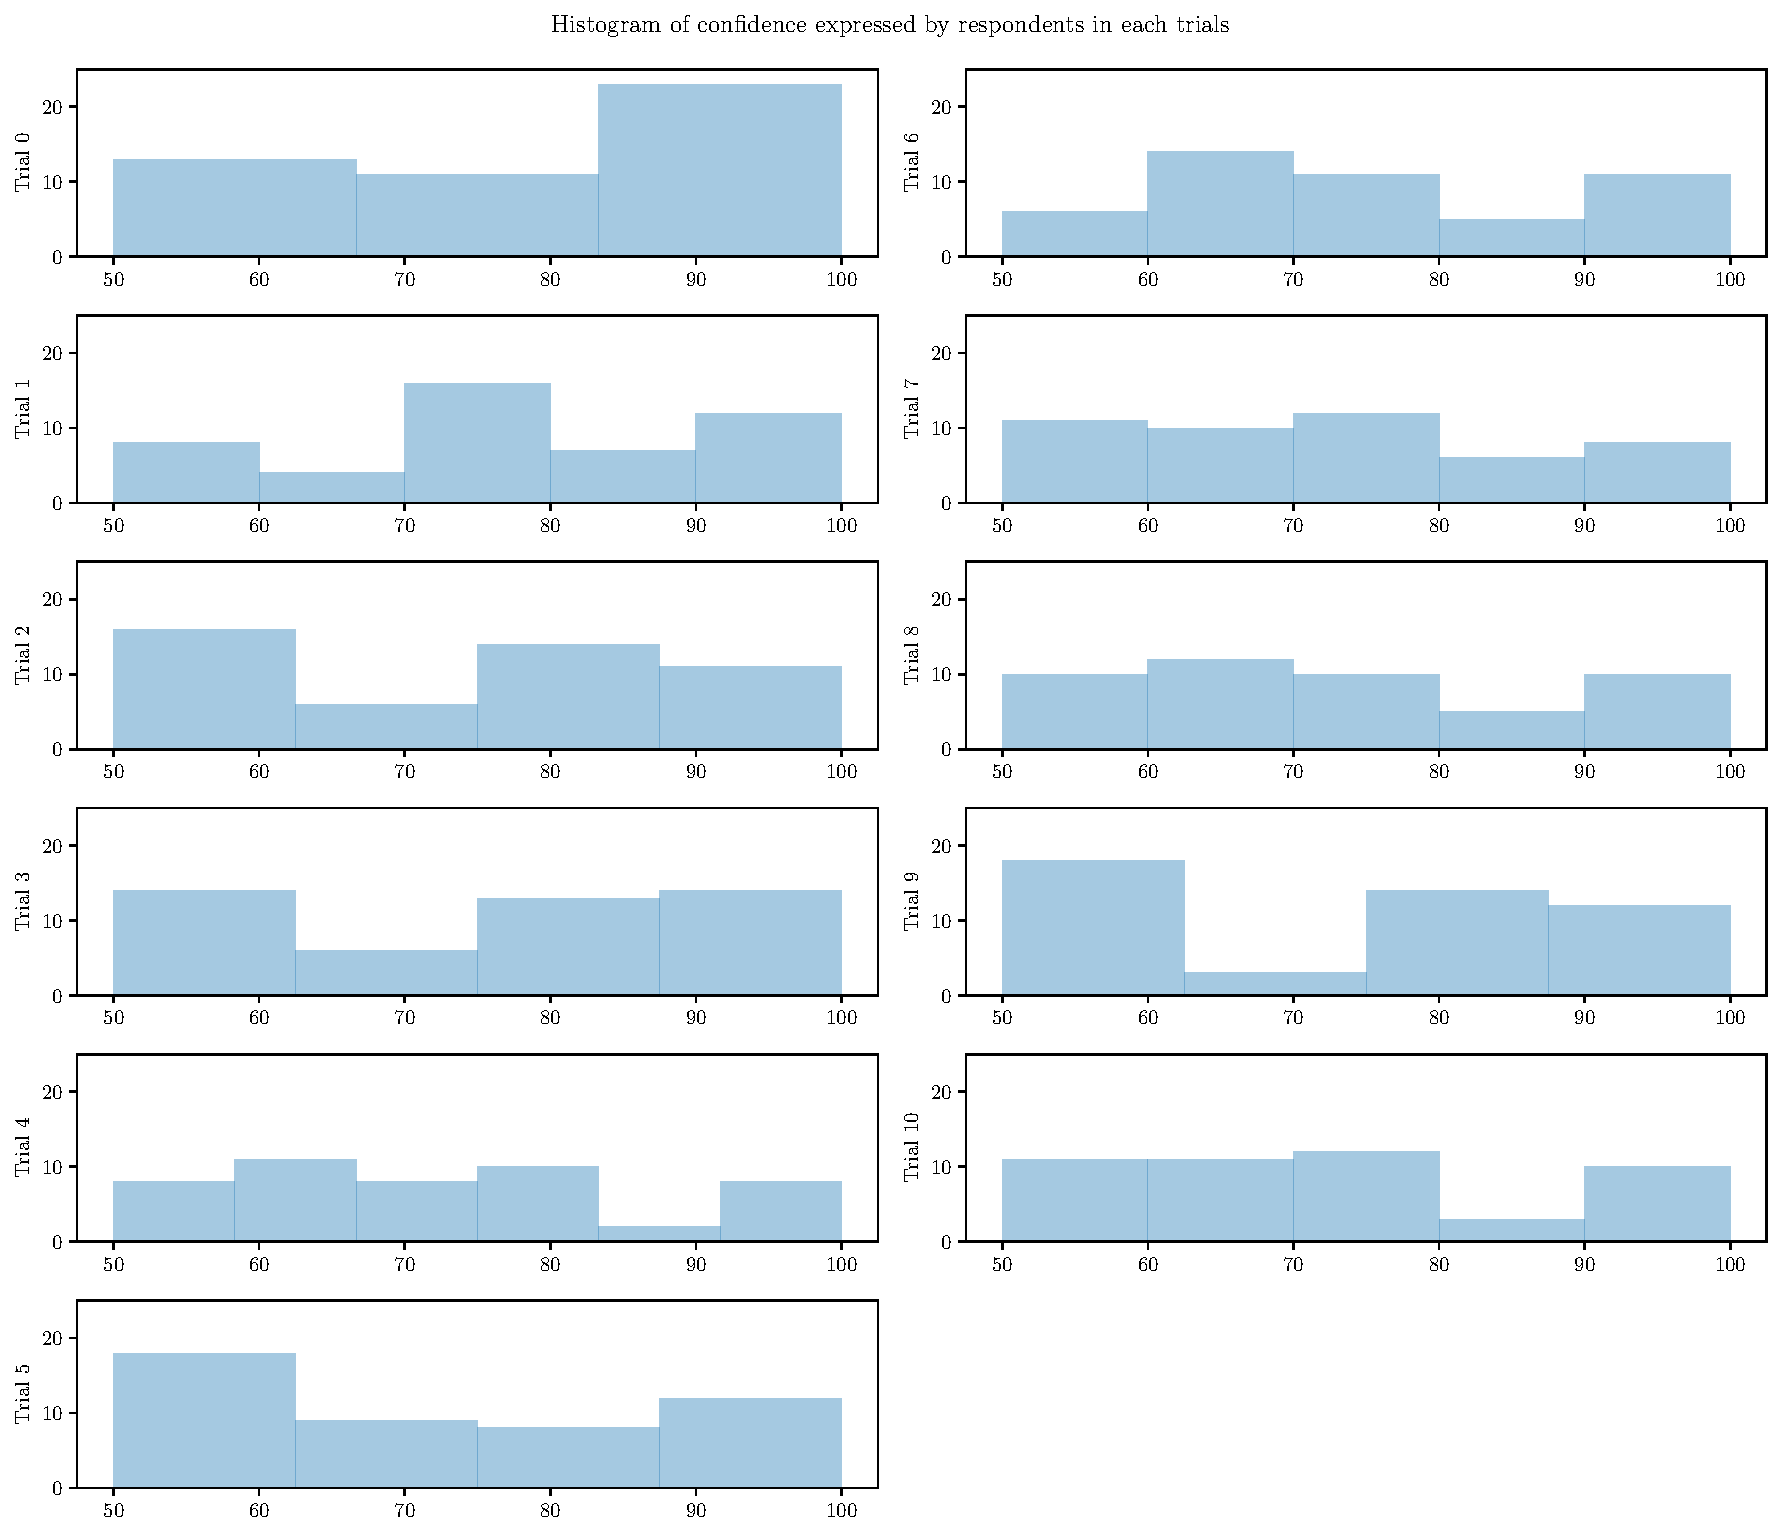
\includegraphics[width=1.5\textwidth]{exp1_conf.pdf}
        }
    \caption{Histogram of confidences in the experiment. Respondents report a wide range of confidence in most questions.}
    \label{fig:conf_hist}
\end{figure}

\newpage
\subsection{Estimation Scores}
We ask the respondents to give us an estimation of others responses to the first question. Specifically, we ask them how much of the respondents, they think, would consider the news piece real.

For the Surprisingly Popular (SP) voting scheme, we need to compare the average estimation for the each of two candidate answer to the actual votes they've gathered. Whichever has a higher share of the votes than was estimated (on average), is the surprisingly popular scheme.

Figure \ref{fig:exp1_estim_trial0} shows the histogram  of estimations, divided into two partitions --- based on the actual vote of participants.
\begin{figure}[H]
    \centering
    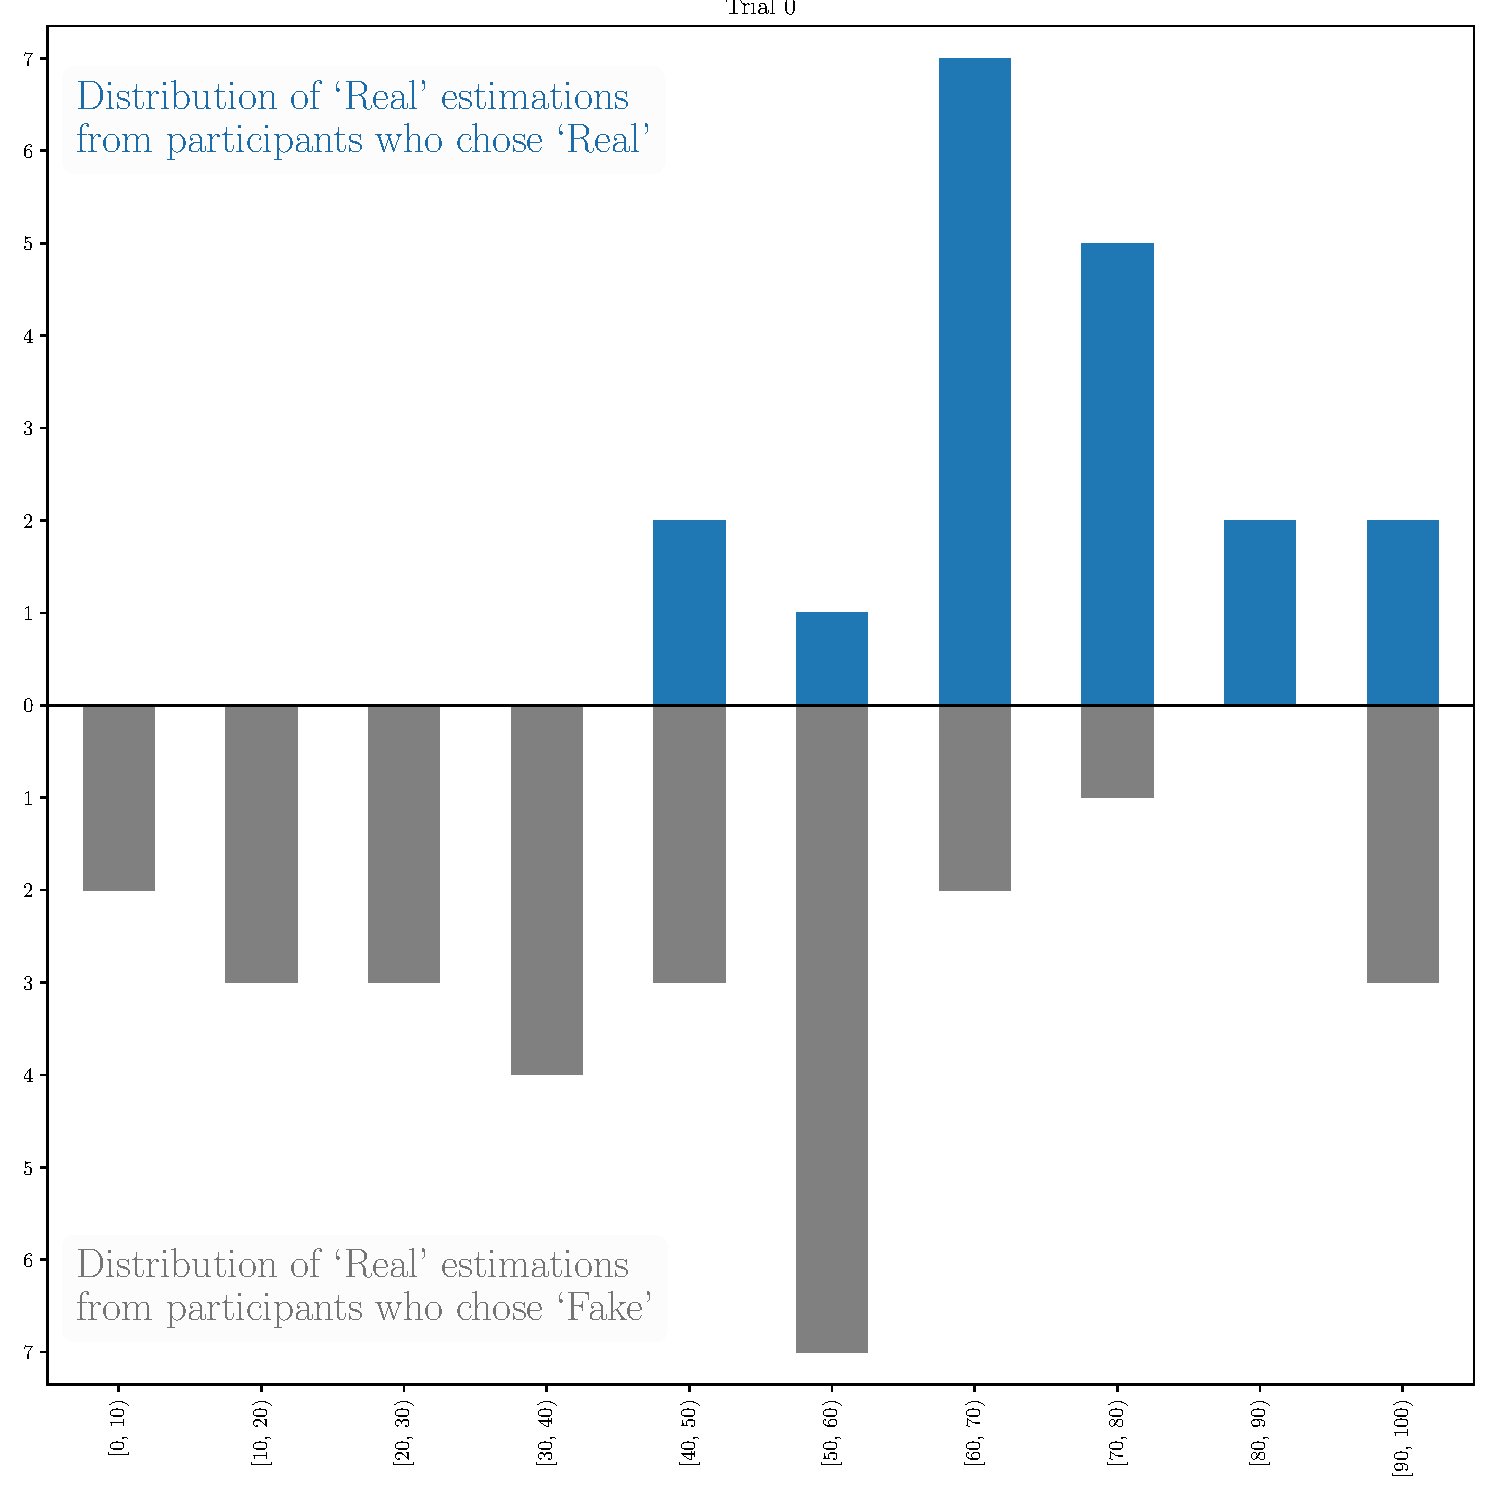
\includegraphics[width=\textwidth]{exp1_estim_trial0.pdf}
    \caption{Estimation histogram for Trial 0. The histograms has been divided into two partitions, depending on the actual vote of participants.}
    \label{fig:exp1_estim_trial0}
\end{figure}

\subsection{Surprisingly Popular and Estimation Scores}
The intuition behind the SP voting mechanism is that either the `experts' (those who know the true answer to the 'real'/'fake' question) are in the majority, or if they are a minority, they know it themselves-- in the sense that they estimate that a majority of the population would choose the opposite of what they have chosen.

If neither of these conditions are met, the mechanism fails to detect the true answer. The SP tries to assign as much weight as possible to the \emph{experts} in the population, even when they are in a minority. As such, the failure of SP signals the lack of expert opinion in the population. 

Figure \ref{fig:exp1_estim_all} shows histograms for all trials. SP fails in trials in trials 0, 1, 3, 5 and 8. In Trial 0, the `experts' are in minority but they are seemingly unaware of this, since they still estimate that a majority will favor their position. Similarly in Trial 1, the experts (those who have chosen 'fake') estimate that most of the population would also think that the news is fake. The analysis for trials 5 and 8 are similar. 

In Trial 3, the experts seem to be in a majority, but their majority is not strong enough to compensate for the fact they too are over-estimating the population. However the difference is very small and with some minor filtering of the noisy data, such a situation can be avoided.

\begin{figure}
    \centering
    \centerline{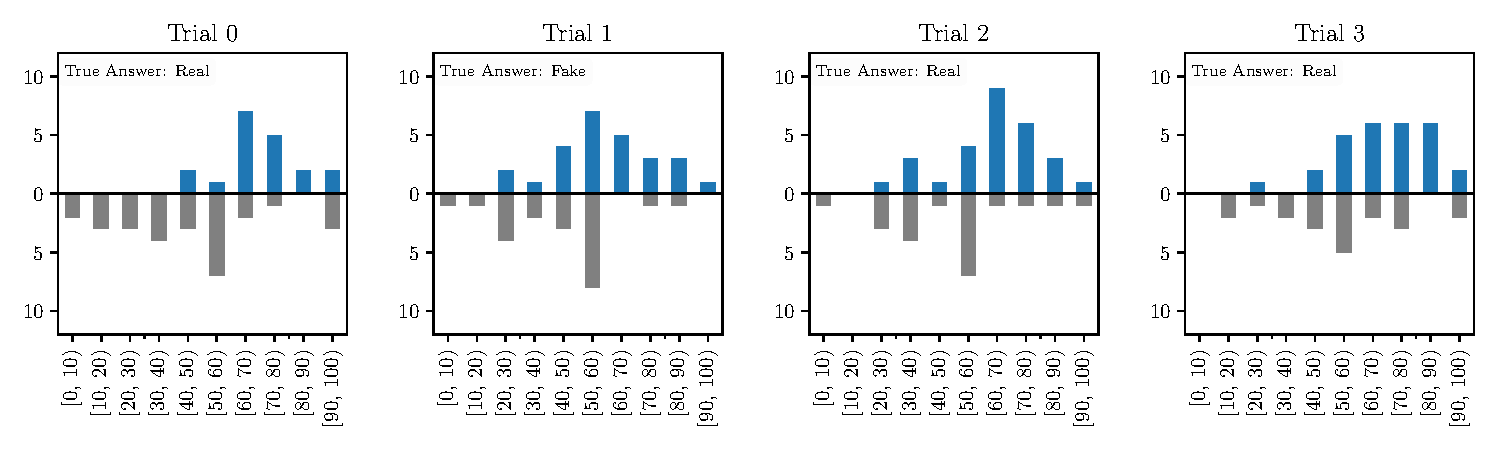
\includegraphics[width=1.5\textwidth]{exp1_estim_0-3.pdf}}
    \centerline{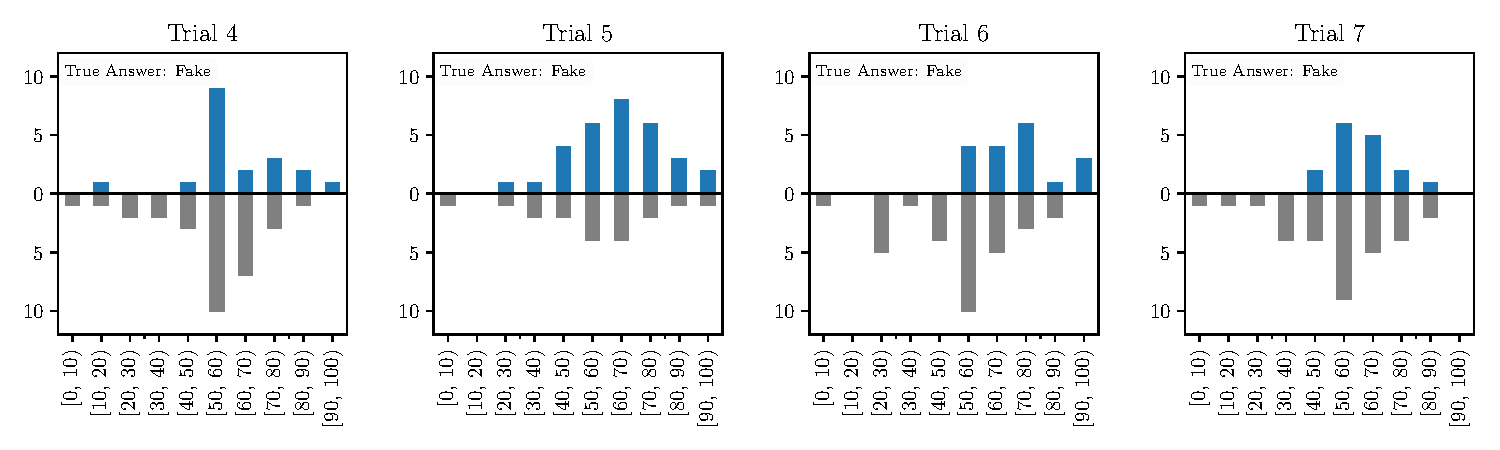
\includegraphics[width=1.5\textwidth]{exp1_estim_4-7.pdf}}
    \centerline{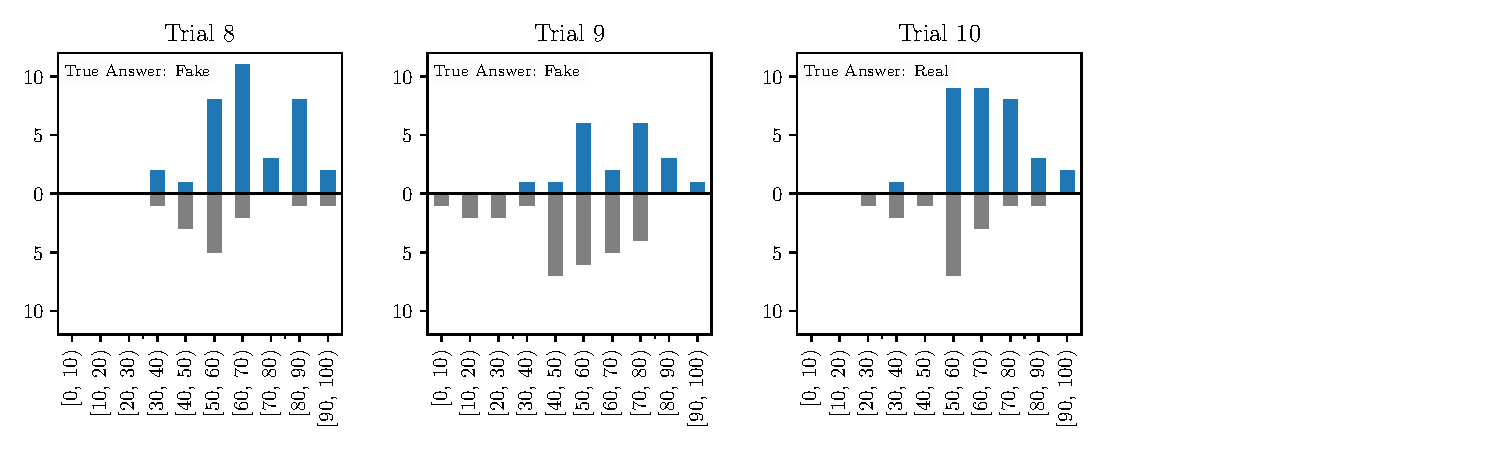
\includegraphics[width=1.5\textwidth]{exp1_estim_8-10.pdf}}
    \caption{Estimation histograms for all trials. For the SP mechanism to work, 'those who know' (who choose the right answer) should either be in the majority themselves or else estimate that 'those who don't know are in the majority'. Without any filtering of the data, SP fails in trials 0, 1, 3, 5 and 8 because neither of these conditions hold. The data is too noisy, as respondents have not taken the time to assess others' potential response.}
    \label{fig:exp1_estim_all}
\end{figure}


% \chapter{Questionnaire Guide}
% \section{Options}
% For each news page shown to you in the following questionnaire, please answer the following questions:

% \begin{enumerate}[label=(\alph*)]
%     \item Is this news item true? True/False
%     \item How confident are you in your answer? Please state your answer either in
%     \begin{itemize}
%         \item Odds using the fractional format with the numerator for the true and the denominator for the false, i.e. $1/100$ (in favour of false), \emph{or}
%         \item Decimal format, i.e., $dec(100/101)  \approx 0.99$ for the same example. (Note that your confidence can logically be between 50\% to 100\%.)
%     \end{itemize}
%     \item In your opinion, what percentage of other people thought that the news item was true?
% \end{enumerate}

% \section{Determination of bonus}
% After the study is complete, we will calculate two accuracy scores for each respondent. 


% \begin{enumerate}
% \item Your objective accuracy score is based on your answers to (a) and (b).
% For each statement we calculate the probability that you think the statement is true and use this, together with whether the statement is actually true to calculate your score. We use the Brier scoring function, which is designed so that your score is maximized when you report your true guess and confidence level. Below is a table which helps you understand the score you would receive, depending on whether your answer in (a) was correct or incorrect. The table gives the score at intervals of ten percentage points, but you can choose any percentage between 50\% and 100\%.

% \begin{table}[H]
%  \centering
% \begin{tabular}{ccc}
% \toprule
%     Your confidence   &   Score if (a) correct   &  Score if (a) incorrect\\
% \midrule
%     50\%              &   0                       &  0 \\
%     60\%              &   9                       &  -11 \\
%     70\%              &   16                      &  -24 \\
%     80\%              &   21                      &  -39 \\
%     90\%              &   24                      &  -56 \\
%     100\%             &   25                      &  -75 \\
% \bottomrule
% \end{tabular}
% \end{table}


% Points to note:
% \begin{itemize}
% \item the more certain you claim to be, the more points you can win
% \item as you approach 100\%, the penalty for being incorrect climbs much faster than the gains for being correct.
% \end{itemize}

% A tip:
% \begin{itemize}
%     \item In the long run, you will score the most points if the numbers correspond to your true levels of confidence. Expressing too much confidence is a common mistake in this game.
% \end{itemize}

% \item Your prediction accuracy score is based on your answers to (c).
% Your prediction accuracy score reflects how well you have predicted the actual percentages of respondents who answered Yes to each of the fifty questions, and how well you have estimated the average confidence levels.

% \end{enumerate}













% \clearpage 
 
% \chapter*{Sample Questions}
% \chapter{WIT News}


 \printbibliography

\end{document}
